Screenshots of UI for the "/learn" page. The live version can be viewed at \url{https://colourful-k-center.herokuapp.com/learn}.

\begin{figure}[H]
    \begin{subfigure}{0.5\textwidth}
        \centering
        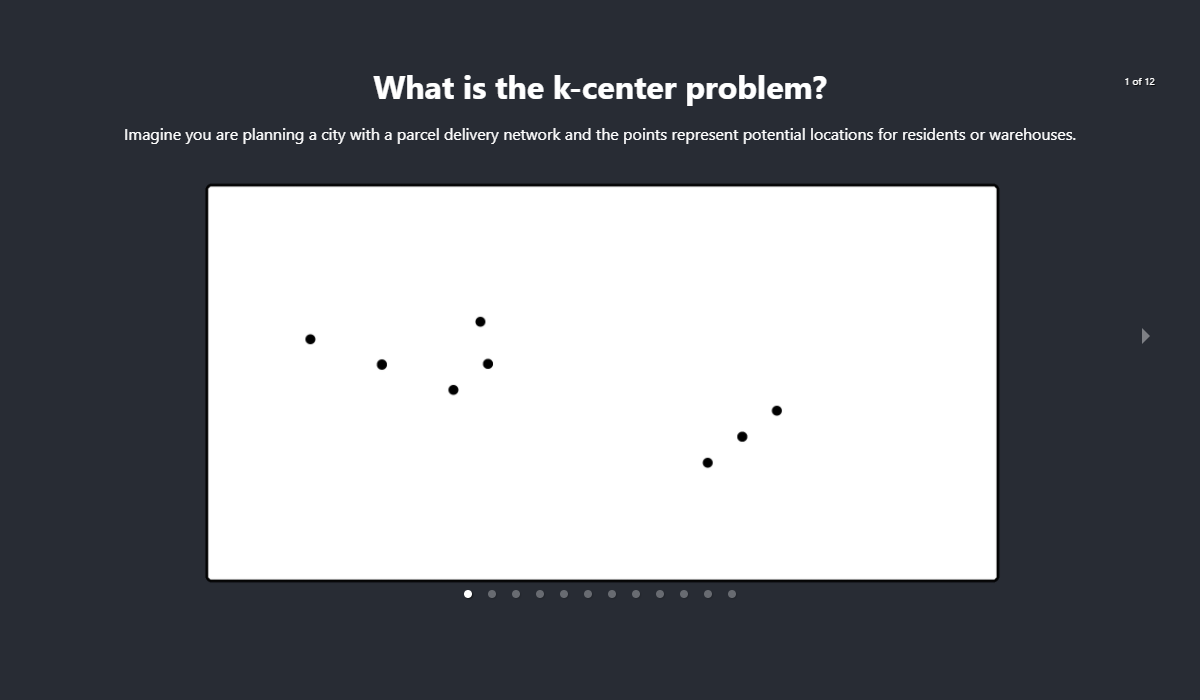
\includegraphics[width=\textwidth]{images/learn_00-base.png}
        \caption{slide 1}
    \end{subfigure}
    \vspace{0.75cm}
    \begin{subfigure}{0.5\textwidth}
        \centering
        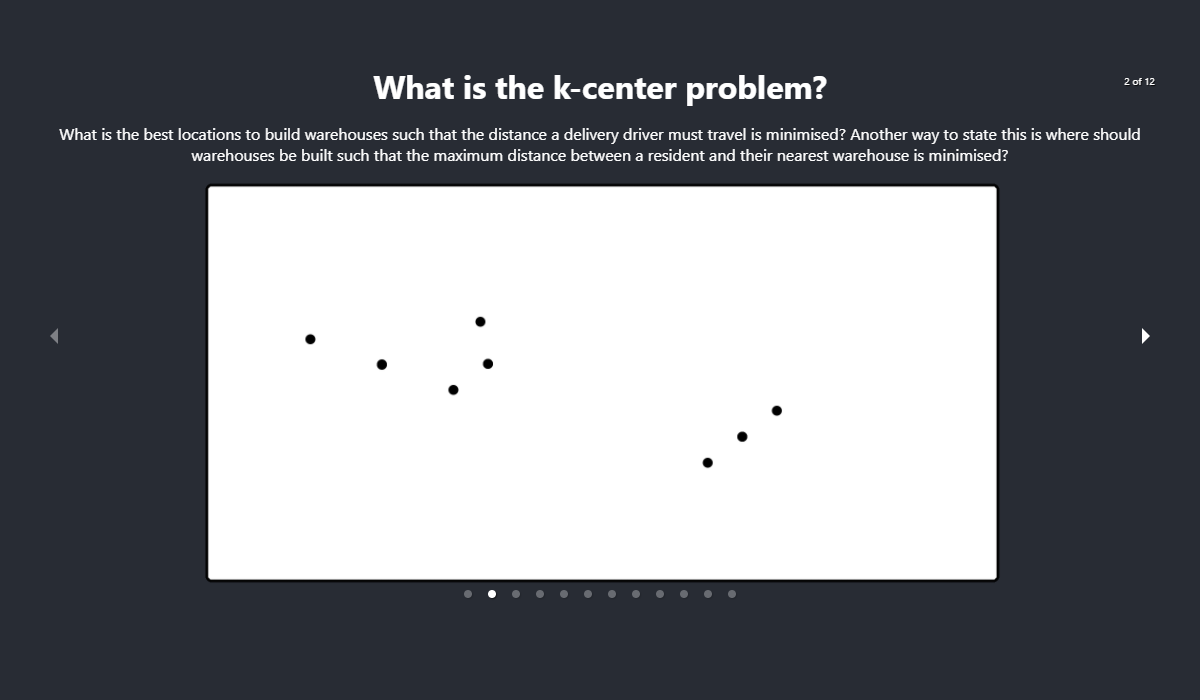
\includegraphics[width=\textwidth]{images/learn_01-base.png}
        \caption{slide 2}
    \end{subfigure}
    \vspace{0.75cm}
    \begin{subfigure}{0.5\textwidth}
        \centering
        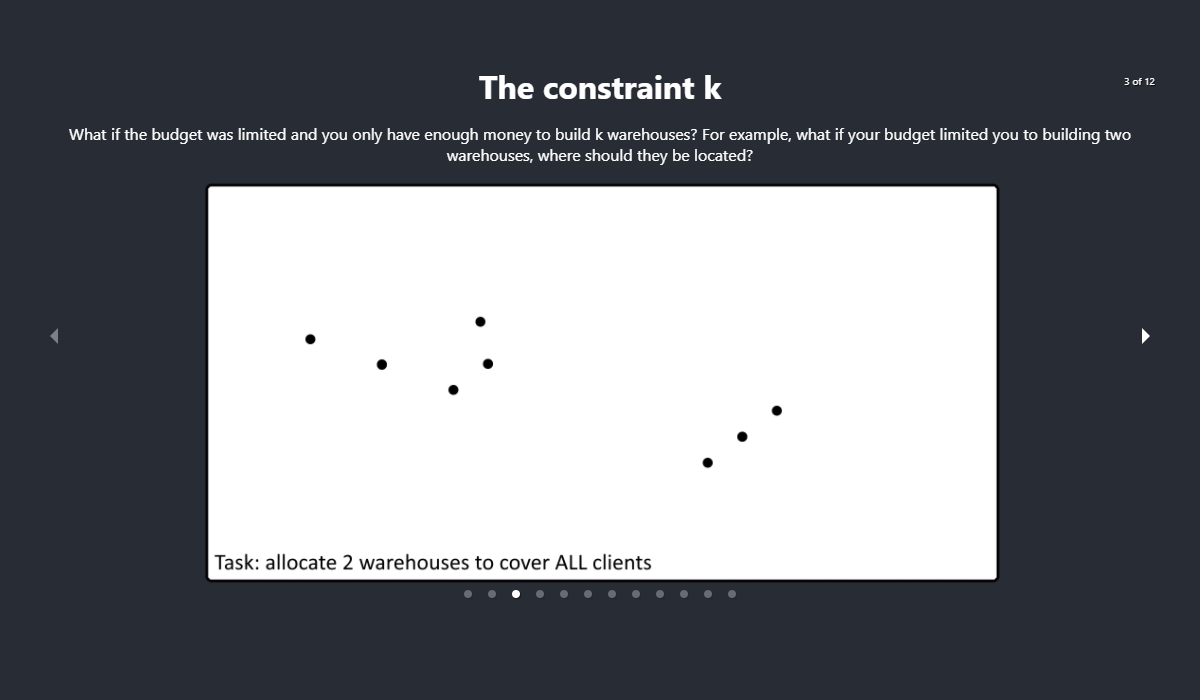
\includegraphics[width=\textwidth]{images/learn_02-base.png}
        \caption{slide 3}
    \end{subfigure}
    \begin{subfigure}{0.5\textwidth}
        \centering
        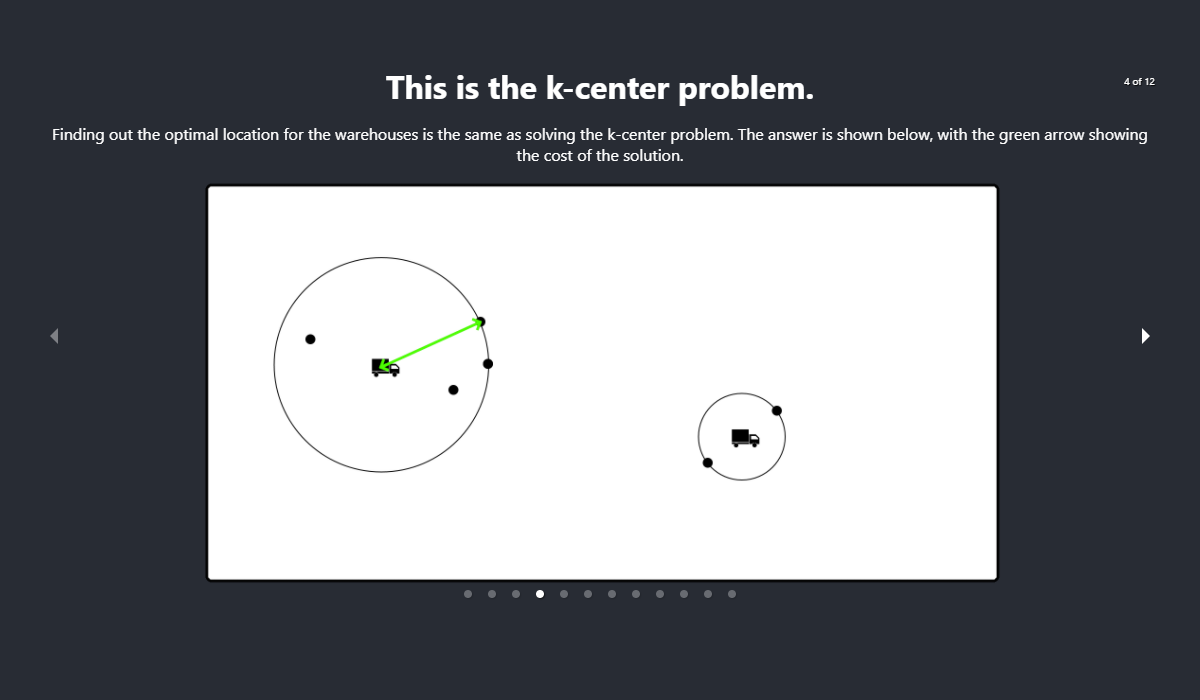
\includegraphics[width=\textwidth]{images/learn_03-base.png}
        \caption{slide 4}
    \end{subfigure}
    \begin{subfigure}{0.5\textwidth}
        \centering
        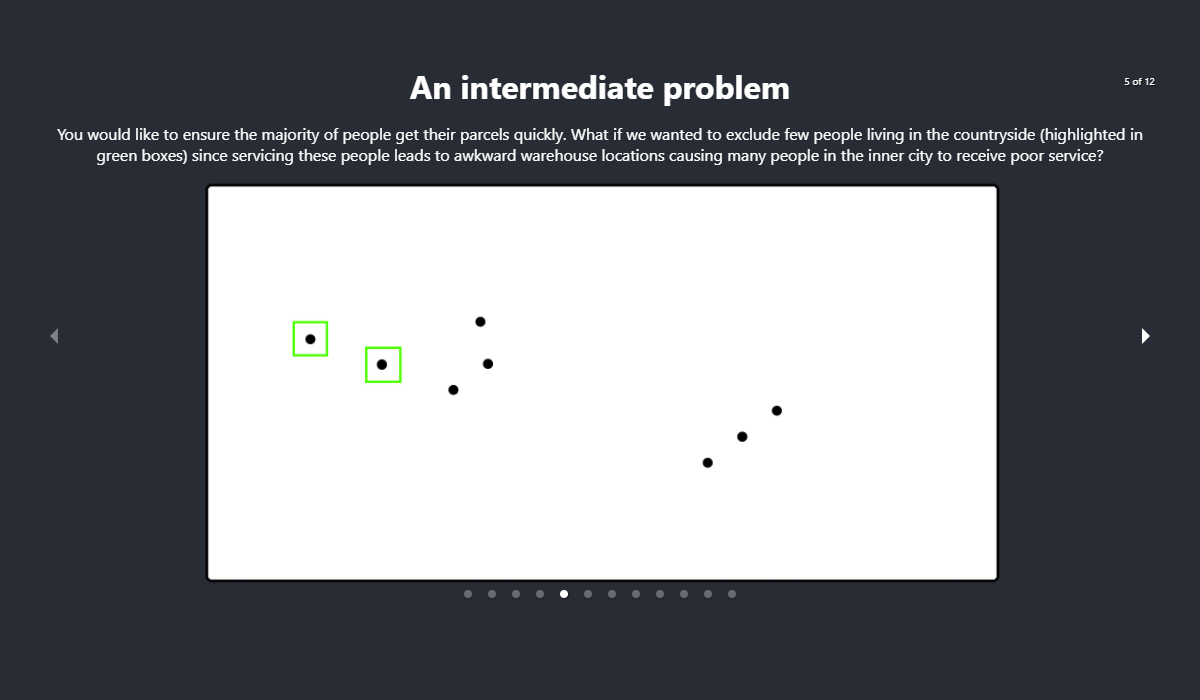
\includegraphics[width=\textwidth]{images/learn_04-base.png}
        \caption{slide 5}
    \end{subfigure}
    \begin{subfigure}{0.5\textwidth}
        \centering
        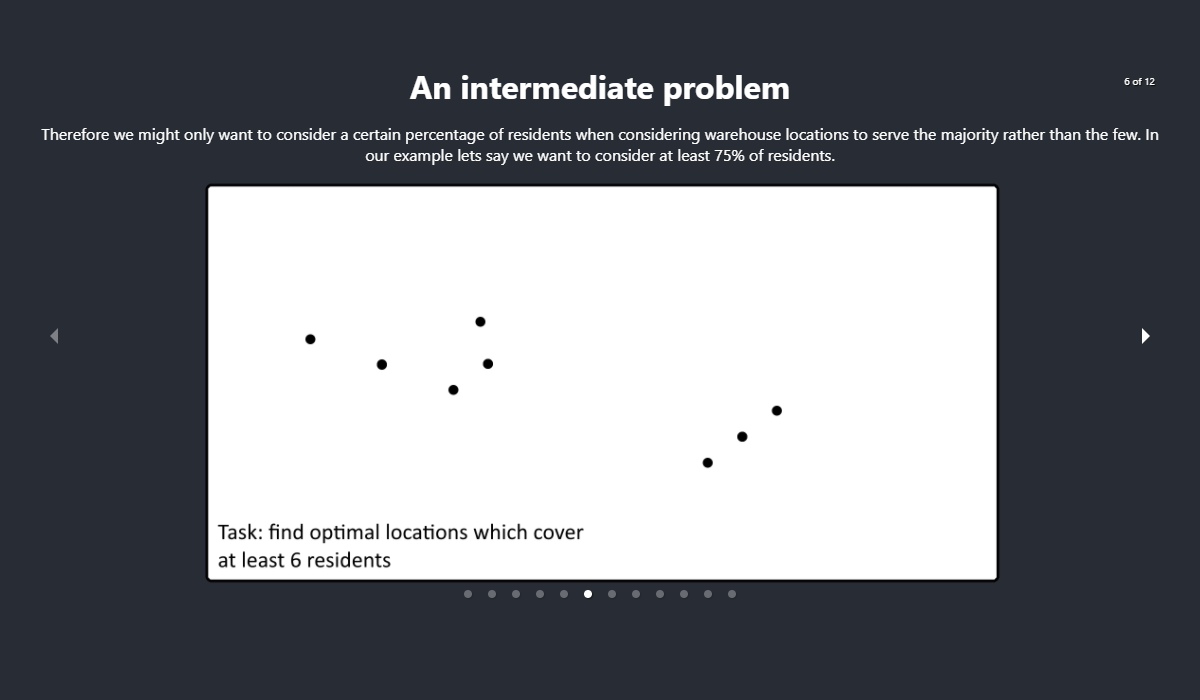
\includegraphics[width=\textwidth]{images/learn_05-base.png}
        \caption{slide 6}
    \end{subfigure}
\end{figure}

\begin{figure}[H]\ContinuedFloat
    \begin{subfigure}{0.5\textwidth}
        \centering
        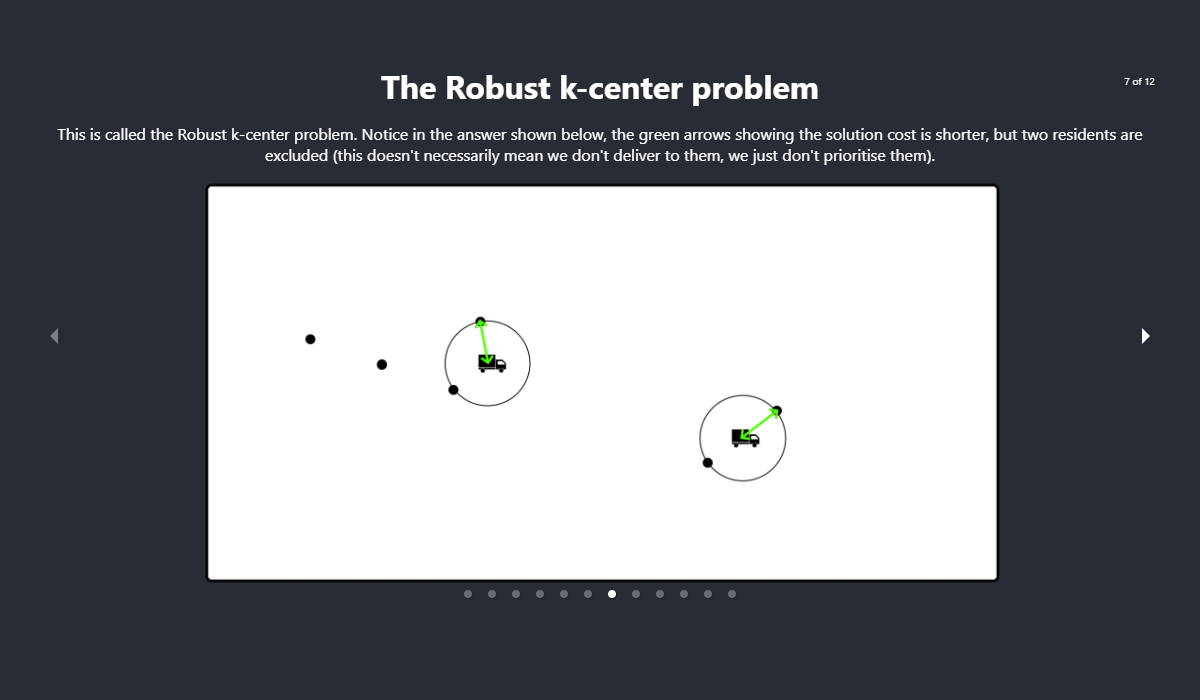
\includegraphics[width=\textwidth]{images/learn_06-base.png}
        \caption{slide 7}
    \end{subfigure}
    \vspace{0.75cm}
    \begin{subfigure}{0.5\textwidth}
        \centering
        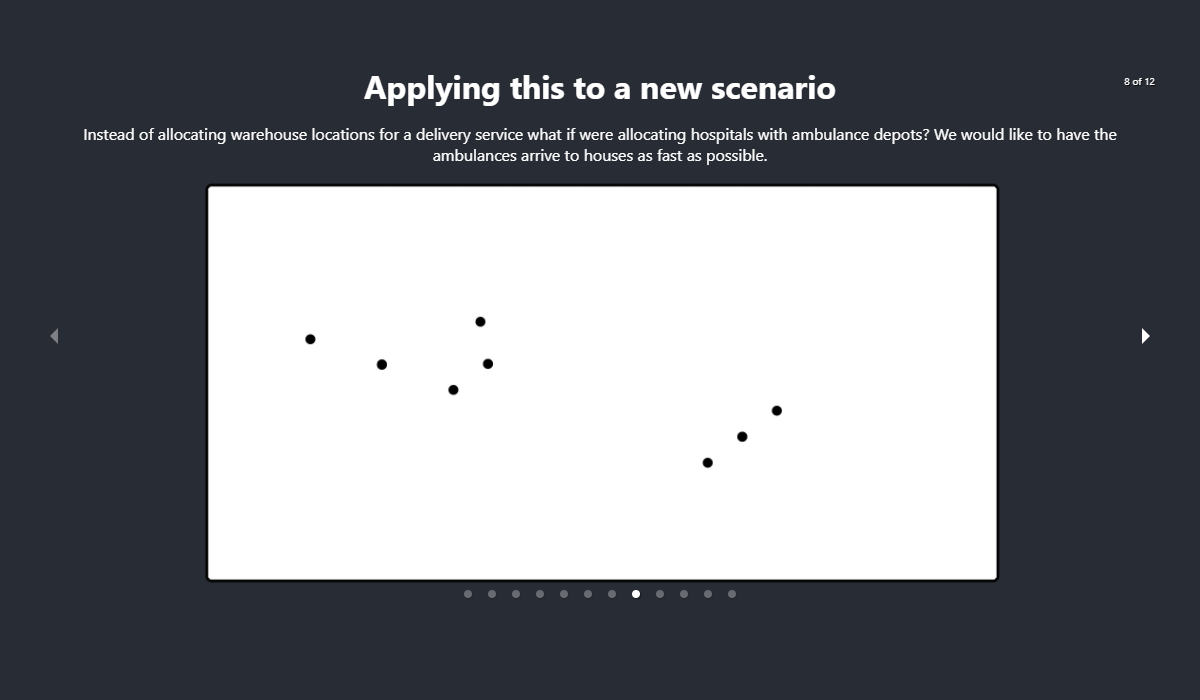
\includegraphics[width=\textwidth]{images/learn_07-base.png}
        \caption{slide 8}
    \end{subfigure}
    \vspace{0.75cm}
    \begin{subfigure}{0.5\textwidth}
        \centering
        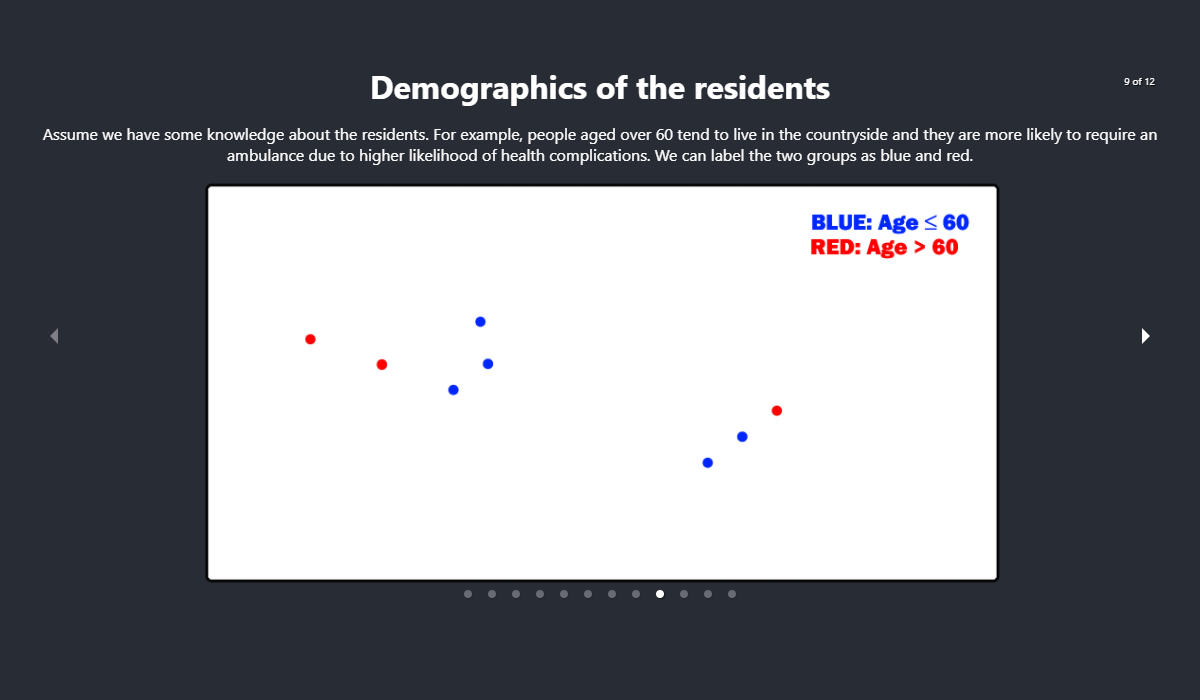
\includegraphics[width=\textwidth]{images/learn_08-base.png}
        \caption{slide 9}
    \end{subfigure}
    \begin{subfigure}{0.5\textwidth}
        \centering
        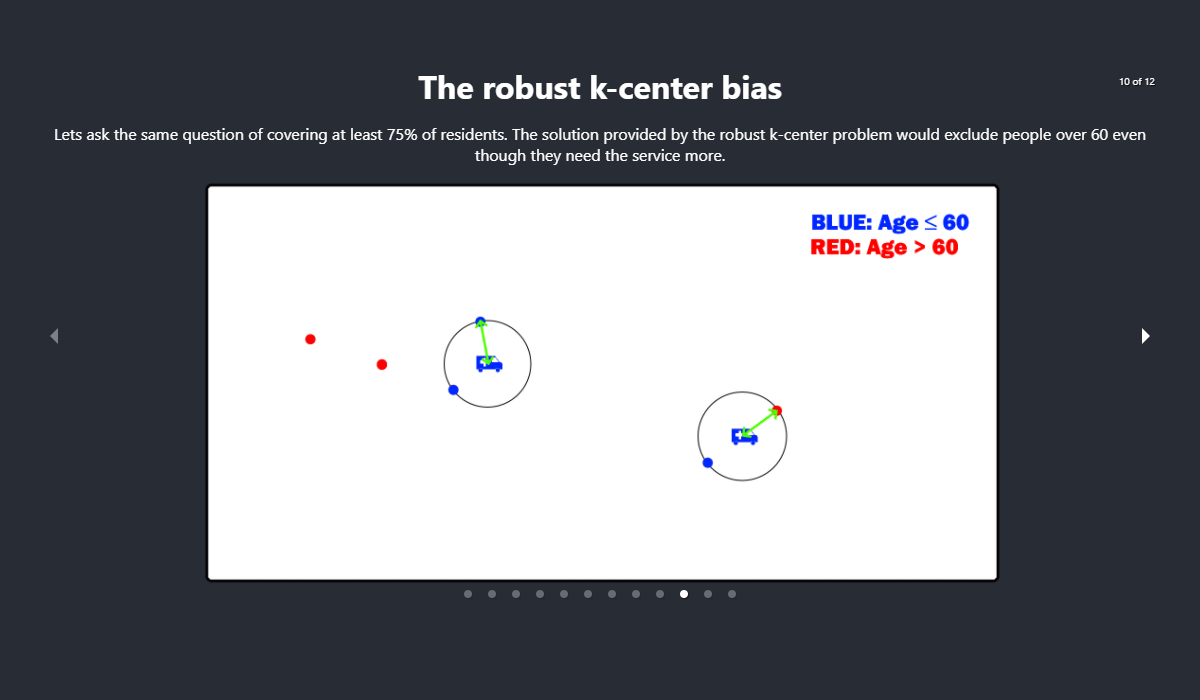
\includegraphics[width=\textwidth]{images/learn_09-base.png}
        \caption{slide 10}
    \end{subfigure}
    \begin{subfigure}{0.5\textwidth}
        \centering
        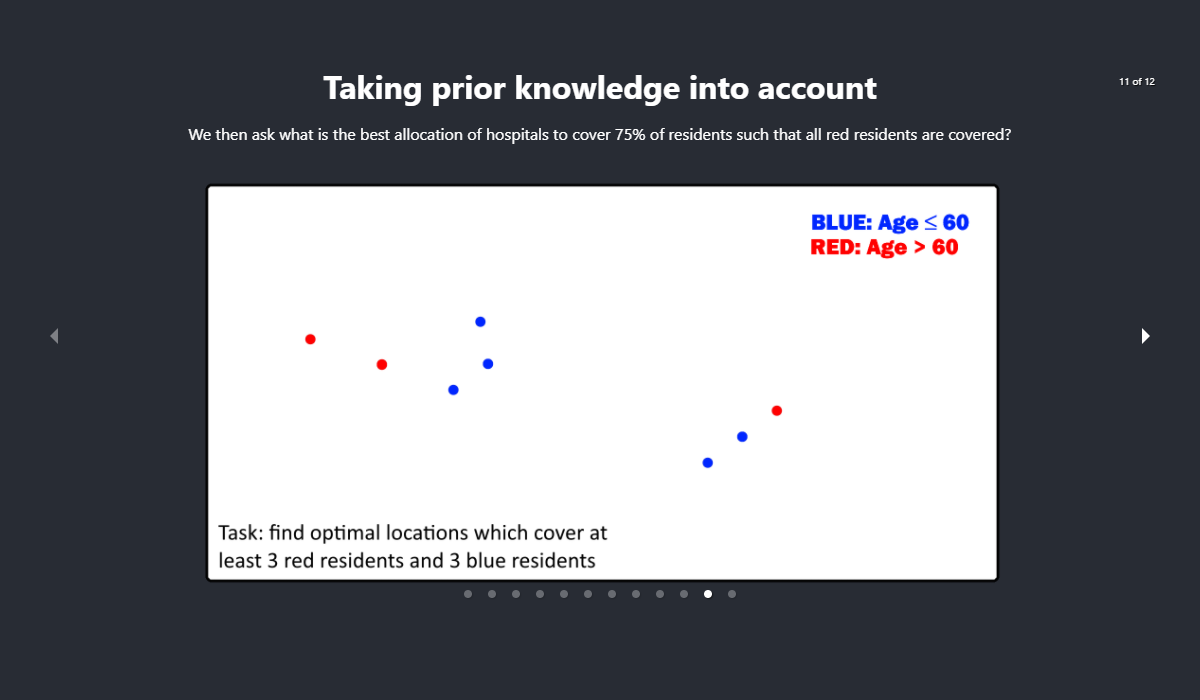
\includegraphics[width=\textwidth]{images/learn_10-base.png}
        \caption{slide 11}
    \end{subfigure}
    \begin{subfigure}{0.5\textwidth}
        \centering
        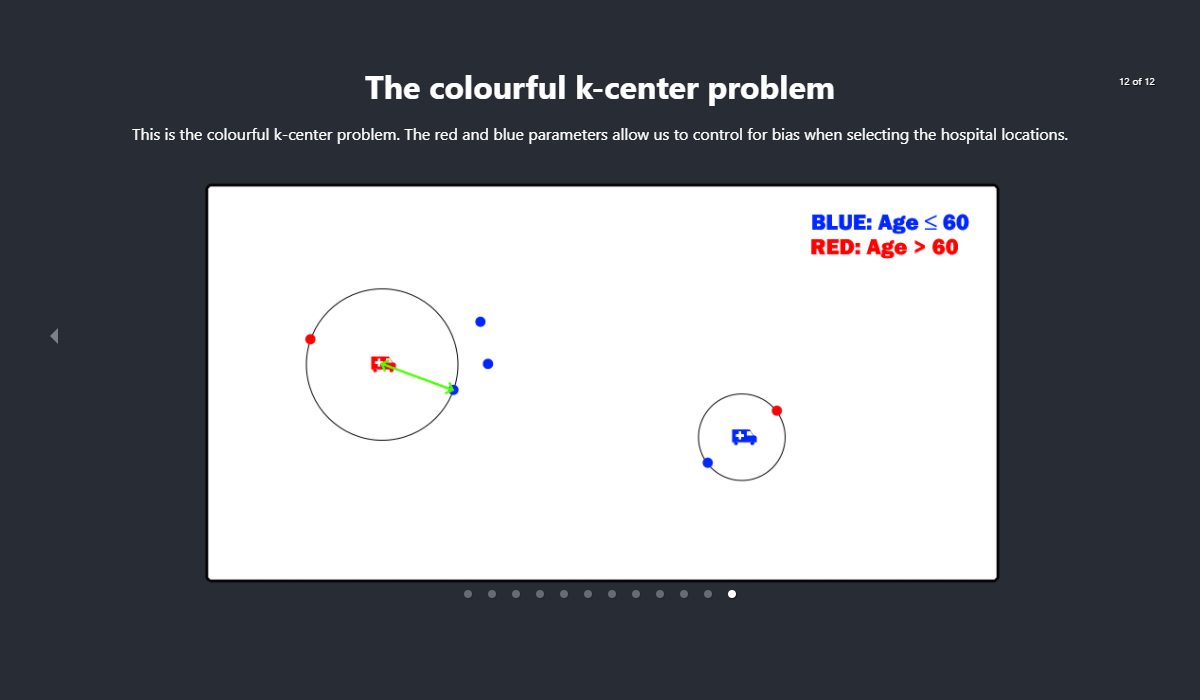
\includegraphics[width=\textwidth]{images/learn_11-base.png}
        \caption{slide 12}
    \end{subfigure}
\end{figure}